\documentclass[10pt, aspectratio=169]{beamer}
\usetheme{metropolis}
\usepackage[utf8]{inputenc}
\usepackage{tikz}
\usepackage{xcolor}

% TikZ libraries
\usetikzlibrary{shapes.geometric, arrows.meta, positioning, shadows}

% Custom colors
\definecolor{gardqblue}{RGB}{79, 195, 247}
\definecolor{gardqgreen}{RGB}{129, 199, 132}
\definecolor{gardqorange}{RGB}{255, 183, 77}
\definecolor{neo4jgreen}{RGB}{0, 140, 201}

% Title information
\title{GARDQ System Overview}
\subtitle{Graph Augmented Retrieval for Data Quality}
\author{Development Team Presentation}
\date{\today}

% Node styles
\tikzstyle{mainnode} = [rectangle, rounded corners, minimum width=2.5cm, minimum height=1cm, text centered, draw=black, fill=gardqblue!20, font=\small]
\tikzstyle{datanode} = [rectangle, rounded corners, minimum width=2cm, minimum height=0.8cm, text centered, draw=black, fill=gardqgreen!20, font=\small]
\tikzstyle{processnode} = [rectangle, rounded corners, minimum width=2.5cm, minimum height=0.8cm, text centered, draw=black, fill=gardqorange!20, font=\small]
\tikzstyle{arrow} = [thick,->,>=stealth]

\begin{document}

% Title slide
\begin{frame}
    \titlepage
\end{frame}

% Slide 1: System Architecture
\begin{frame}{System Architecture}
    \begin{center}
    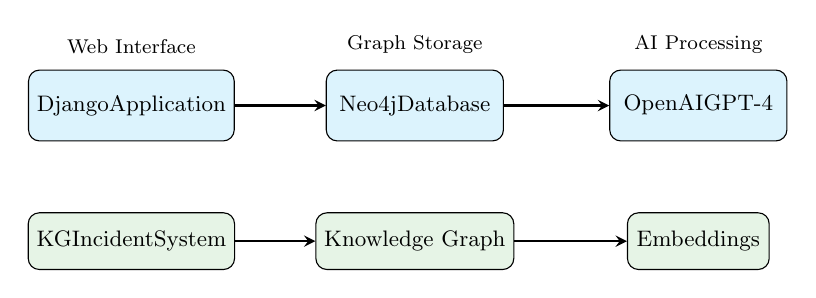
\begin{tikzpicture}[scale=0.9, transform shape]
        % Main components
        \node[mainnode] (django) at (0,0) {Django\\Application};
        \node[mainnode] (neo4j) at (4,0) {Neo4j\\Database};
        \node[mainnode] (openai) at (8,0) {OpenAI\\GPT-4};
        
        % Sub-components
        \node[datanode, below=1cm of django] (kg) {KGIncidentSystem};
        \node[datanode, below=1cm of neo4j] (graph) {Knowledge Graph};
        \node[datanode, below=1cm of openai] (embeddings) {Embeddings};
        
        % Connections
        \draw[arrow] (django) -- (neo4j);
        \draw[arrow] (neo4j) -- (openai);
        \draw[arrow] (kg) -- (graph);
        \draw[arrow] (graph) -- (embeddings);
        
        % Labels
        \node[above=0.1cm of django, font=\footnotesize] {Web Interface};
        \node[above=0.1cm of neo4j, font=\footnotesize] {Graph Storage};
        \node[above=0.1cm of openai, font=\footnotesize] {AI Processing};
    \end{tikzpicture}
    \end{center}
    
    \vspace{0.5cm}
    \begin{itemize}
        \item Django handles incident submission and visualization
        \item Neo4j stores tickets as structured knowledge graph
        \item OpenAI provides analysis and solution generation
    \end{itemize}
\end{frame}

% Slide 2: Knowledge Graph Construction (Based on Paper)
\begin{frame}{Knowledge Graph Construction}
    \begin{columns}[T]
        \begin{column}{0.5\textwidth}
            \textbf{Dual-Level Architecture:}
            \begin{enumerate}
                \footnotesize
                \item \textbf{Intra-ticket Tree} $\mathcal{T}_i(\mathcal{N}, \mathcal{E}, \mathcal{R})$
                \begin{itemize}
                    \scriptsize
                    \item Node $(i,s)$: section $s$ of ticket $t_i$
                    \item Tree structure for each ticket
                    \item Sections: Summary, Description, Solution, etc.
                \end{itemize}
                \item \textbf{Inter-ticket Graph} $\mathcal{G}(\mathcal{T}, \mathcal{E}, \mathcal{R})$
                \begin{itemize}
                    \scriptsize
                    \item Explicit links $\mathcal{E}_{exp}$ (parent/clone)
                    \item Implicit links $\mathcal{E}_{imp}$ (similarity)
                    \item $cos(embed(\mathcal{T}_i), embed(\mathcal{T}_j)) \geq \theta$
                \end{itemize}
            \end{enumerate}
            
            \vspace{0.3cm}
            \textbf{Hybrid Construction Method:}
            \begin{itemize}
                \footnotesize
                \item Rule-based extraction for predefined fields
                \item LLM parsing for complex text sections
                \item Guided by YAML template $\mathcal{T}_{template}$
            \end{itemize}
        \end{column}
        
        \begin{column}{0.5\textwidth}
            \begin{center}
            \begin{tikzpicture}[scale=0.65, transform shape]
                % Intra-ticket structure
                \node[mainnode] (t1) at (0,0) {ENT-22970};
                \node[datanode, minimum width=1.2cm] (s1) at (-1,-1.2) {Summary};
                \node[datanode, minimum width=1.2cm] (s2) at (1,-1.2) {Solution};
                
                % Clone ticket
                \node[mainnode] (t2) at (4,0) {PORT-133061};
                \node[datanode, minimum width=1.2cm] (s3) at (3,-1.2) {Summary};
                \node[datanode, minimum width=1.2cm] (s4) at (5,-1.2) {Solution};
                
                % Similar tickets
                \node[mainnode] (t3) at (2,-3) {ENT-1744};
                
                % Relations
                \draw[arrow] (t1) -- (s1);
                \draw[arrow] (t1) -- (s2);
                \draw[arrow] (t2) -- (s3);
                \draw[arrow] (t2) -- (s4);
                
                % Explicit clone link
                \draw[arrow, thick, color=gardqred] (t1) -- node[above, font=\tiny] {clone} (t2);
                
                % Implicit similarity
                \draw[arrow, dashed, <->] (t1) -- node[left, font=\tiny] {similar} (t3);
            \end{tikzpicture}
            \end{center}
            
            \textbf{Construction Formula:}
            \footnotesize
            $$t_i = t_{i,rule} \cup t_{i,llm}$$
            $$\mathcal{T}_i = \text{RuleParse}(t_{i,rule}) + \text{LLMParse}(t_{i,llm})$$
        \end{column}
    \end{columns}
\end{frame}

% Slide 3: Query Processing Pipeline
\begin{frame}{Query Processing: 4-Step Pipeline}
    \begin{center}
    \begin{tikzpicture}[scale=0.75, transform shape, node distance=1.5cm]
        % Step 1
        \node[processnode, minimum width=3.5cm] (step1) at (0,0) {1. Query Analysis};
        \node[below=0.2cm of step1, font=\tiny, text=gardqgray] {Extract entities \& intents};
        
        % Step 2
        \node[processnode, minimum width=3.5cm, right=of step1] (step2) {2. Ticket Retrieval};
        \node[below=0.2cm of step2, font=\tiny, text=gardqgray] {Cosine similarity search};
        
        % Step 3
        \node[processnode, minimum width=3.5cm, below=1.5cm of step1] (step3) {3. Subgraph Extraction};
        \node[below=0.2cm of step3, font=\tiny, text=gardqgray] {Cypher query generation};
        
        % Step 4
        \node[processnode, minimum width=3.5cm, right=of step3] (step4) {4. Response Generation};
        \node[below=0.2cm of step4, font=\tiny, text=gardqgray] {Context-aware solution};
        
        % Arrows
        \draw[arrow] (step1) -- (step2);
        \draw[arrow] (step2) -- (step3);
        \draw[arrow] (step3) -- (step4);
    \end{tikzpicture}
    \end{center}
    
    \vspace{0.5cm}
    \begin{columns}[T]
        \begin{column}{0.5\textwidth}
            \textbf{Steps 1-2: Find Relevant Tickets}
            \begin{itemize}
                \footnotesize
                \item Parse query for entities/intents
                \item Calculate embedding similarity
                \item Retrieve top-K tickets (K=10)
                \item Filter by similarity threshold (>0.5)
            \end{itemize}
        \end{column}
        \begin{column}{0.5\textwidth}
            \textbf{Steps 3-4: Extract \& Generate}
            \begin{itemize}
                \footnotesize
                \item Generate Cypher query dynamically
                \item Extract ticket subgraphs
                \item Aggregate context from similar tickets
                \item Generate solution with references
            \end{itemize}
        \end{column}
    \end{columns}
\end{frame}

% Slide 4: Similarity Calculation & Why Graph > Traditional RAG
\begin{frame}{Similarity Calculation \& Graph Advantages}
    \begin{columns}[T]
        \begin{column}{0.5\textwidth}
            \textbf{Two-Level Similarity Calculation:}
            
            \textbf{1. During Graph Build (Offline)}
            \begin{itemize}
                \scriptsize
                \item Calculate cosine similarity between all ticket pairs
                \item Using SUMMARY embeddings (384-dim)
                \item Formula: $\frac{emb_i \cdot emb_j}{||emb_i|| \times ||emb_j||}$
                \item Create SIMILAR\_TO relation if score $\geq$ 0.8
                \item Store similarity score in relationship
            \end{itemize}
            
            \textbf{2. During Query (Online)}
            \begin{itemize}
                \scriptsize
                \item Generate query embedding
                \item Search sections with \texttt{gds.similarity.cosine()}
                \item Compare with ALL section types
                \item Take MAX similarity per ticket
                \item Filter: similarity > 0.5
                \item Return top-K tickets with scores
            \end{itemize}
        \end{column}
        
        \begin{column}{0.5\textwidth}
            \textbf{Graph Advantages vs Traditional RAG:}
            
            \textbf{1. Pre-computed Relationships}
            \begin{itemize}
                \scriptsize
                \item SIMILAR\_TO relations already exist
                \item No need to compute all similarities at query time
                \item Can traverse similarity network efficiently
            \end{itemize}
            
            \textbf{2. Rich Context Extraction}
            \begin{itemize}
                \scriptsize
                \item Not just nearest neighbors
                \item Include related tickets via graph traversal
                \item Aggregate solutions from ticket clusters
            \end{itemize}
            
            \textbf{3. Structured Information}
            \begin{itemize}
                \scriptsize
                \item Sections maintain semantic meaning
                \item Entities provide categorical filtering
                \item Relations enable pattern discovery
            \end{itemize}
            
            \begin{alertblock}{Key Insight}
                \footnotesize
                Traditional RAG: "Find similar text chunks"\\
                Graph RAG: "Find similar tickets + their network"
            \end{alertblock}
        \end{column}
    \end{columns}
\end{frame}

% Slide 5: Implementation Details
\begin{frame}{Implementation in GARDQ}
    \begin{columns}[T]
        \begin{column}{0.5\textwidth}
            \textbf{Technical Stack:}
            \begin{itemize}
                \footnotesize
                \item \textbf{Backend}: Django web framework
                \item \textbf{Graph DB}: Neo4j with Cypher queries
                \item \textbf{AI/ML}: OpenAI GPT-4o-mini
                \item \textbf{Embeddings}: Sentence-transformers (384-dim)
            \end{itemize}
            
            \vspace{0.3cm}
            \textbf{Key Files:}
            \begin{itemize}
                \footnotesize
                \item \texttt{kg\_knowledge\_system.py} - Core logic
                \item \texttt{migrate\_to\_kg.py} - Graph construction
                \item \texttt{views.py} - Web endpoints
                \item \texttt{templates/} - UI components
            \end{itemize}
        \end{column}
        
        \begin{column}{0.5\textwidth}
            \textbf{Data Flow:}
            \begin{center}
            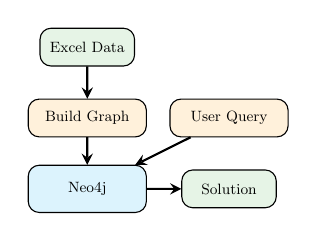
\begin{tikzpicture}[scale=0.6, transform shape]
                \node[datanode] (excel) at (0,0) {Excel Data};
                \node[processnode] (build) at (0,-1.5) {Build Graph};
                \node[mainnode] (neo4j) at (0,-3) {Neo4j};
                \node[processnode] (query) at (3,-1.5) {User Query};
                \node[datanode] (result) at (3,-3) {Solution};
                
                \draw[arrow] (excel) -- (build);
                \draw[arrow] (build) -- (neo4j);
                \draw[arrow] (query) -- (neo4j);
                \draw[arrow] (neo4j) -- (result);
            \end{tikzpicture}
            \end{center}
            
            \textbf{Web Interface:}
            \begin{itemize}
                \footnotesize
                \item \texttt{/} - Incident submission
                \item \texttt{/metrics/} - Graph statistics
                \item \texttt{/kg-visualization/} - Graph view
            \end{itemize}
        \end{column}
    \end{columns}
\end{frame}



\end{document}